% !TEX root = ../main.tex

\chapter{\label{section:evaluation}Inférer le retard subi}

% \mtctitle{}
% \minitoc

% Dans les chapitres précedents nous avons généré un large ensemble de données pour évaluer l'ampleur du problème des interférences sur notre cible matérielle et caractériser l'activité mémoire.
% Dans les chapitres précedents, nous avons, d'une part, introduit un ensemble de microbenchmarks couvrant un large spectre de sensibilité aux interférences, et, d'autre part, défini des métriques caractérisant le comportement des applications en isolation.
Dans les chapitres précédents, nous avons introduit des microbenchmarks couvrant un large spectre de sensibilité aux interférences et un ensemble de métriques caractérisant leur comportement en isolation.
Grâce à ces deux outils, nous disposons d'une grande quantité de données sur la relation entre ce comportement et cette sensibilité.
Dans ce chapitre, nous nous penchons sur l'utilisation de ces données pour capturer le comportement de notre plateforme matériel.
Le but étant de pouvoir prédire le retard subi par un programme sans avoir à injecter de charges.
Pour cela, nous allons nous reposer sur des algorithmes d'apprentissage automatique pour apprendre le comportement du matériel à partir des données dont nous disposons.
Par la même occasion, nous allons évaluer quelles métriques sont pertinentes pour caractériser la sensibilité aux interférences.
%Nous allons, pour cela, utiliser des techniques d'apprentissages automatique.


Ce chapitre comprend deux sections.
Dans la première, nous présenterons l'algorithme d'apprentissage que nous utilisons.
Dans la seconde, nous procéderons à l'évaluation proprement dite, nous y présenterons d'abord les applications utilisées pour entrainer et valider les résultats de l'algorithme de régression, puis les différents ensembles de caractéristiques évalués, avant de présenter les résultats de l'évaluation.

\section{Algorithme d'apprentissage}

% Nous avons recours à des techniques d'apprentissage automatique pour inférer le retards subi par une application à partir de ses caractéristiques de comportement en isolation.
Le but d'un algorithme d'apprentissage est d'approximer une fonction à partir de données.
On cherche donc à construire une fonction $f$ dont le but est de prédire la valeur d'une variable $y$ à partir d'un vecteur de caractéristiques $X$. 

$$y = f(X)$$

La nature de la variable $y$ détermine le type de problème que l'on essaie de résoudre. 
Si $y$ appartient à un ensemble fini et discret, on parle de \emph{classification}.
Un exemple de problème classification est de déterminer si une image représente un objet en particulier.
Dans le cas où $y$ appartient à un ensemble continu, on parle de \emph{régression}.
Par exemple, un modèle climatique prédisant l'évolution de la température moyenne sur terre résout un problème de régression.
Nous cherchons à prédire le surcoût temporel subi par une application à cause des interférences.
L'ensemble des surcoûts que peut subir une application étant continu
%~\footnote{Ce n'est pas vrai \emph{stricto senso}. En effet, le temps dans un ordinateur étant discret, le surcoût temporelle tel que nous l'avons défini ne peut être qu'un nombre rationel. L'ensemble des surcoût temporelles possibles est donc un sous ensemble des nombre rationels, qui est discret. Ce détail n'affectant pas le résultat final, nous approximons le surcoût par un nombre réel.}
, il s'agit donc d'un problème de régression.


Dans ce chapitre, nous étudions la qualité de la prédiction que l'on peut obtenir en fonction de la nature de ce vecteur, c'est-à-dire les différentes caractéristiques de trafic que nous utilisons pour faire la prédiction. L'apprentissage que nous effectuons est \emph{supervisé}.
La construction de la fonction d'inférence se fait à l'aide d'un ensemble de données d'entrainement qui consiste en un ensemble de données étiquetées, qui sont des couples $(X, y)$ issus de mesures.

Nous utilisons des forêts d'arbre de décisions pour inférer le retard subi par une application à partir de caractéristiques de leur comportement.
Nous avons choisi cet algorithme, car il est à la fois relativement résistant au problème du surapprentissage et simple à utiliser.
Le reste de cette section présente brièvement cet algorithme.
Nous commencerons par présenter les arbres de décisions qui sont fondamentaux pour la mise en œuvre de celui-ci.
Puis nous nous pencherons sur l'algorithme des forêts aléatoires lui-même.

\subsection{\label{section:inference:reg:decision-tree}Arbre de décisions}

Un arbre de décision est une suite de conditions sur une variable d'entrée $X$ permettant de décider d'une valeur $y$.
Les valeurs de $y$ sont les feuilles de l'arbre, et les conditions sur $X$ ses embranchements.
La construction d'un tel arbre à partir d'un ensemble de données est une méthode d'apprentissage permettant de résoudre aussi bien des problèmes de régressions que de classifications.~\cite{breiman2017classification}.

% TODO figures.

La construction d'un arbre de décision est décrite dans l'algorithme~\ref{alg:decision_tree}.
Elle consiste à découper \emph{récursivement de façon gloutonne} l'ensemble de données d'entrainement en sous-ensemble homogène.
L'algorithme prend en entrée un jeu de donnée $D$ et un compteur de profondeur $L$.
Si les données dans $D$ sont suffisamment homogènes, ou si la hauteur de l'arbre dépasse un seuil préalablement fixé, alors le découpage s'arrête et une feuille est retournée.
Sinon une \emph{coupe} est effectuée pour déterminer une condition séparant le jeu de données en deux, et l'algorithme est appliqué récursivement sur les deux sous-ensembles résultant de cette coupe

\begin{algorithm}
\begin{algorithmic}

\Function{BuildTree}{$(D, L)$}
  \If{$L \ge L_{max} \wedge Impurity(D) \le I_{min}$}
  	\State{\Return $Leaf(D)$}
  \EndIf

  \State{}

  \State{$C \gets bestSplit(D)$}
  
  \State{}
  
  \State{$D_L \gets C(D)$}
  \State{$D_R \gets \neg C(D)$}

  \State{}
  
  \State{$T_L \gets BuildTree(D_L, L+1)$}
  \State{$T_R \gets BuildTree(D_R, L+1)$}
  
  \State{}

  \State{\Return $Branch(C, T_L, T_R)$}

\EndFunction

\end{algorithmic}
\caption{\label{alg:decision_tree}Entrainement d'un arbre de décision}
\end{algorithm}


Les différentes conditions constituant l'arbre de décisions sont déterminées lors des coupes de l'ensemble de données.
Pour un ensemble de données $D$, une coupe optimale $C$ maximise un critère de gain d'information $IG(D, c)$.
Avant de définir ce critère, il faut introduire la notion d'\emph{impureté.}
L'\emph{impureté} d'un ensemble de données $D$ est une mesure de son hétérogénéité.
Plusieurs critères d'impureté existent, mais pour la régression on utilise la \emph{variance} de $D$.
Si $N$ est le nombre d'éléments de l'ensemble d'entrainement et $\mu$ la moyenne des $y$ dans $D$, alors l'impureté de $D$ est

\begin{equation}
	Impurity(D) = \frac{1}{N} \sum_{i=1}^N(y_i - \mu)^2 
\end{equation}

Un ensemble de données est donc parfaitement homogène lorsque son impureté vaut 0.
Vu qu'il s'agit d'un cas que l'on rencontre rarement pour des ensembles de données de plus d'un élément, 
un ensemble de données est déclaré homogène si son impureté est inférieure ou égale à un seuil $I_{min}$.
Le gain d'information apporté par une coupe $c$ sur des données $D$ est la différence entre l'impureté des données de $D$ et la somme des impuretés pondérées des ensembles résultant de cette coupe.

\begin{equation}
 IG(D, c) = Impurity(D) - \frac{N_{L}}{N}impurity(D_L) -\frac{N_{R}}{N}impurity(D_R)
\end{equation}

Les arbres de décisions ont pour avantage d'être simples à mettre en œuvre et d'être interprétables par un humain.
Mais ils ont pour inconvénient d'être très sensibles au problème de \emph{surapprentissage} (ou \emph{overfitting}).
Cela signifie que la fonction apprise s'adapte trop étroitement aux données d'apprentissage, l'empêchant ainsi de se généraliser à d'autres données(figure~\ref{fig:overfitting}).
Il s'agit d'une fonction de prédiction avec un biais faible, mais une variance très élevée.
On peut réduire cette variance en limitant la hauteur de l'arbre ou à l'aide d'algorithmes randomisés comme les forêts aléatoires.
Cette deuxième approche s'avérant particulièrement efficace c'est celle que nous utilisons. 

\begin{figure}
	\centering
	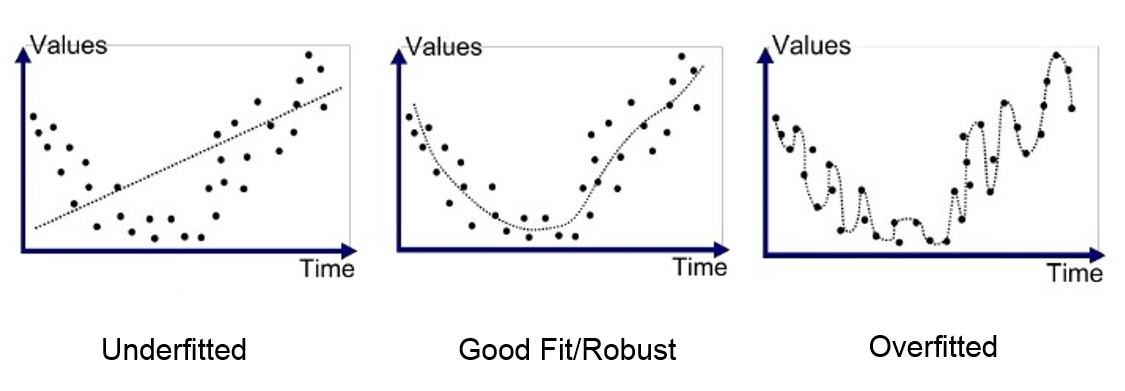
\includegraphics[width=\linewidth]{graphics/figures/overfitting.png}
	\caption{\label{fig:overfitting}Exemples de sousapprentissage, d'apprentissage adapté et de surapprentissage (source~\cite{overfitting})}
\end{figure}


\subsection{Forets aléatoires}

L'algorithme des forêts aléatoires~\cite{breiman2001random} utilise une approche dite d'\emph{ensachage~\cite{breiman1996bagging} (ou bagging\footnote{\textit{B}ootstrap \textit{agg}regat\textit{ing}})} pour rendre les arbres de décisions plus robustes face au problème de surapprentissage.
Il est décrit dans la figure~\ref{fig:random-forest} et peut se résumer en trois étapes:
\begin{enumerate}
	\item \emph{Échantillonnage} $N$ sous-ensemble d'entrainements $D_i$ sont tirés aléatoirement \emph{avec remises} à partir de l'ensemble d'entrainements.
	\item \emph{Décisions} Pour chaque tirage $D_i$ on entraine un arbre de décision $f_i$. l'entrainement est similaire à celui décrit dans la section~\ref{section:inference:reg:decision-tree} à une exception près.
	Soit $p$ le nombre de composantes de $x$ (le nombre de caractéristiques à partir duquel on veut prédire y).
	Plutôt que de choisir une coupe optimale parmi toutes les caractéristiques disponibles, on choisit la coupe optimale pour un ensemble de $p_{try}$ caractéristiques tirées aléatoirement. 
	\item \emph{fusion} pour faire une inférence, on utilise les $n$ estimateurs entrainés durant l'étape précédente et on fusionne leur résultat. 
	Dans le cas d'une procédure de régression, la fusion consiste à prendre la moyenne de la sortie des différents arbres de décisions.
\end{enumerate}

\begin{figure}
	\centering
	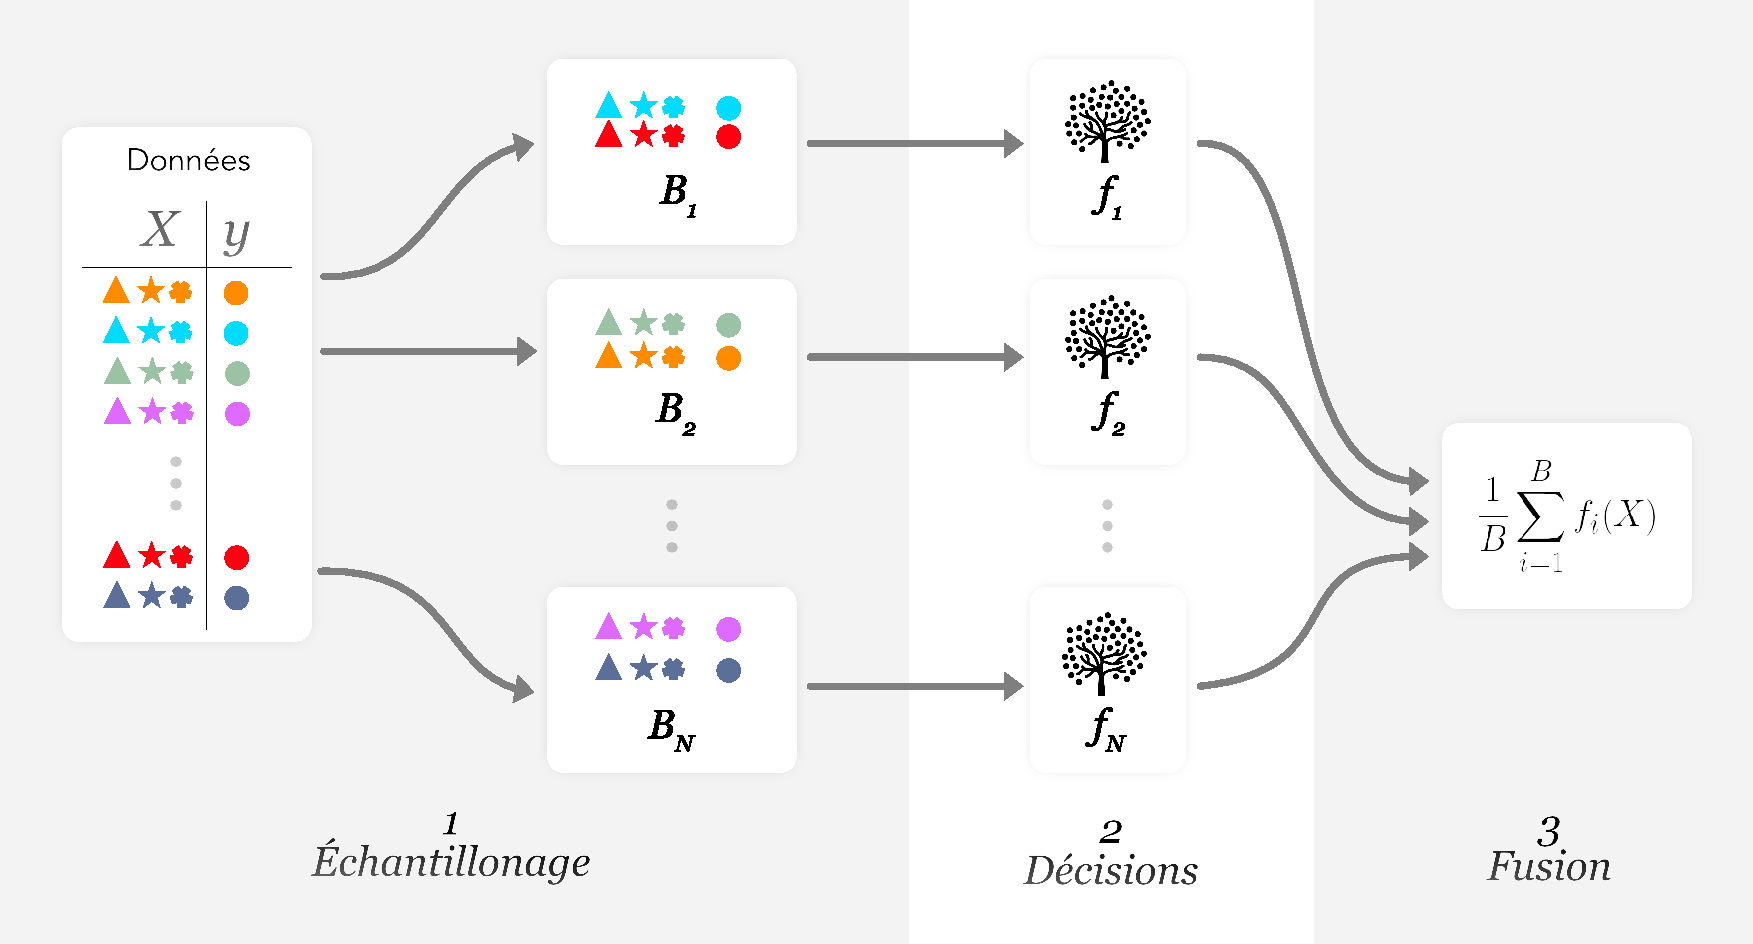
\includegraphics[width=\linewidth]{figures/random-forest.pdf}
	\caption{\label{fig:random-forest}}
\end{figure}

Cet algorithme a l'avantage d'offrir de bons résultats tout en étant simple à utiliser.
Il n'ya en effet que deux paramètres à considérer, le nombre d'arbres $N$ que l'on entraine et le nombre $p_{try}$ de caractéristiques que l'on tire pour déterminer une coupe optimale. 
En règle générale, la valeur de $p_{try}$ utilisée (et celle que nous utilisons~\cite{docrandomforest}) est 
\begin{equation}
	\label{equation:ptry}
	p_{try} = \lfloor \sqrt{p} \rfloor
\end{equation}

% We use a regression algorithm to predict the worst observed overhead suffered by an application given a set of metrics characterizing its behavior in isolation.
% We use the random forests~\cite{breiman2001random} regressor's implementation of the Scikit-learn machine learning library.
% We chose to use random forests because it is well suited for the regression of non-linear models and it is robust against overfitting.
% The training set used to fit the regressor is in charge of capturing the hardware behavior.
% In our evaluation, it consists in the overhead and the characterization in isolation of the set microbenchmark instances presented in section~\ref{section:microbench_eval}.
% The validation set consists in a set of applications from the \textsc{MiBench}~\cite{guthaus2001mibench} and the \textsc{PARSEC}~\cite{bienia2008parsec} suites.
% We use the checkpointing facility  provided by our profiler to split them into phases.
% We do not consider the initialization phases of any application in our experiments.
%

\section{Évaluation}

Nous décrivons maintenant comment nous utilisons l'apprentissage pour inférer le surcoût induit par les interférences.
Nous commençons par présenter les différentes applications utilisées pour entrainer le prédicteur et valider sa précision.
Nous présentons ensuite les différents ensembles de caractéristiques que nous utilisons en entrée pour la prédiction.
Enfin, nous évaluons quels ensembles de caractéristiques sont les plus adaptés pour notre problème.

\subsection{Applications}

Nous décrivons ici les différentes applications utilisées pour évaluer notre approche.
Il y en a deux types: les applications utilisées pour entrainer le modèle de prédiction et celles utilisées pour évaluer la qualité de la prédiction.

\subsubsection{Ensemble d'entrainement}

Les données de l'ensemble d'entrainement sont issues de nos microbenchmarks.
L'ensemble d'entrainement final est en partie constitué de l'ensemble décrit dans la section~\ref{section:microbench_dataset}.
Pour les applications du groupe \texttt{MemBench}, d'autres instances ont été ajoutées.
Ces instances ont des longueurs de rafales 20 et 100.
Les répartitions d'accès évaluées sont identiques.
Les intensités testées suivent la même règle, mais au lieu d'être comprises entre 0 et 10 000, elles sont comprises entre 0 et 2000.

\subsubsection{Ensemble de validation}

L'ensemble utilisé pour valider les données est constitué d'applications appartenant aux suites de benchmarks \textsc{MiBench}~\cite{guthaus2001mibench} et \textsc{PARSEC}~\cite{bienia2008parsec}.

Nous utilisons la fonctionnalité de points de contrôle offerte par notre profileur pour découper les applications en différentes phases.
Le processus de découpage est actuellement manuel.
Il commence par la génération d'un profil haute résolution de l'application, dont l'examen visuel permet d'identifier les différentes phases de l'application.
Nous plaçons ensuite des contrôles dans le code des applications.
Pour cela, nous nous aidons l'outil \texttt{addr2line} pour identifier les lignes de code exécutées dans les phases.
Enfin on vérifie visuellement que les points de contrôles sont bien placés.

Les applications évaluées, ainsi que le nombre de phases pour chacune d'elle est donné par le tableau~\ref{table:appli-validation}.
Les suites de benchmarks sont généralement constituées de petits programmes n'effectuant qu'une action en particulier.
Cela explique que pour beaucoup d'applications, il n'y a qu'une seule phase (comme illustré dans la figure~\ref{fig:adpcm}).
C'est surtout le cas pour les applications issues de la suite MiBench.
Néanmoins, certaines applications sont suffisamment complexes pour avoir plusieurs phases (comme illustré dans la figure~\ref{fig:fluidanimate-small}).

Un des aspects importants qui rentre en compte lorsque l'on identifie les phases est la \emph{granularité} à laquelle on observe le comportement d'accès à la mémoire.
Ce critère détermine notamment la taille des phases.
Des phases courtes permettent, certes, d'isoler plus de comportement que des phases longues, mais apportent deux inconvénients.
D'abord, plus une phase est courte, plus elle impactée par ce qui passé avant qu'elle débute.
Ensuite, effectuer des mesures à grain fin peut être difficile. 
Pour ces raisons, nous avons choisi de limiter la granularité des phases.
Ainsi, nous nous limitons à l'étude de phases de plus de 3 millisecondes.

\begin{figure}
	\begin{subfigure}[t]{\linewidth}
		\centering
		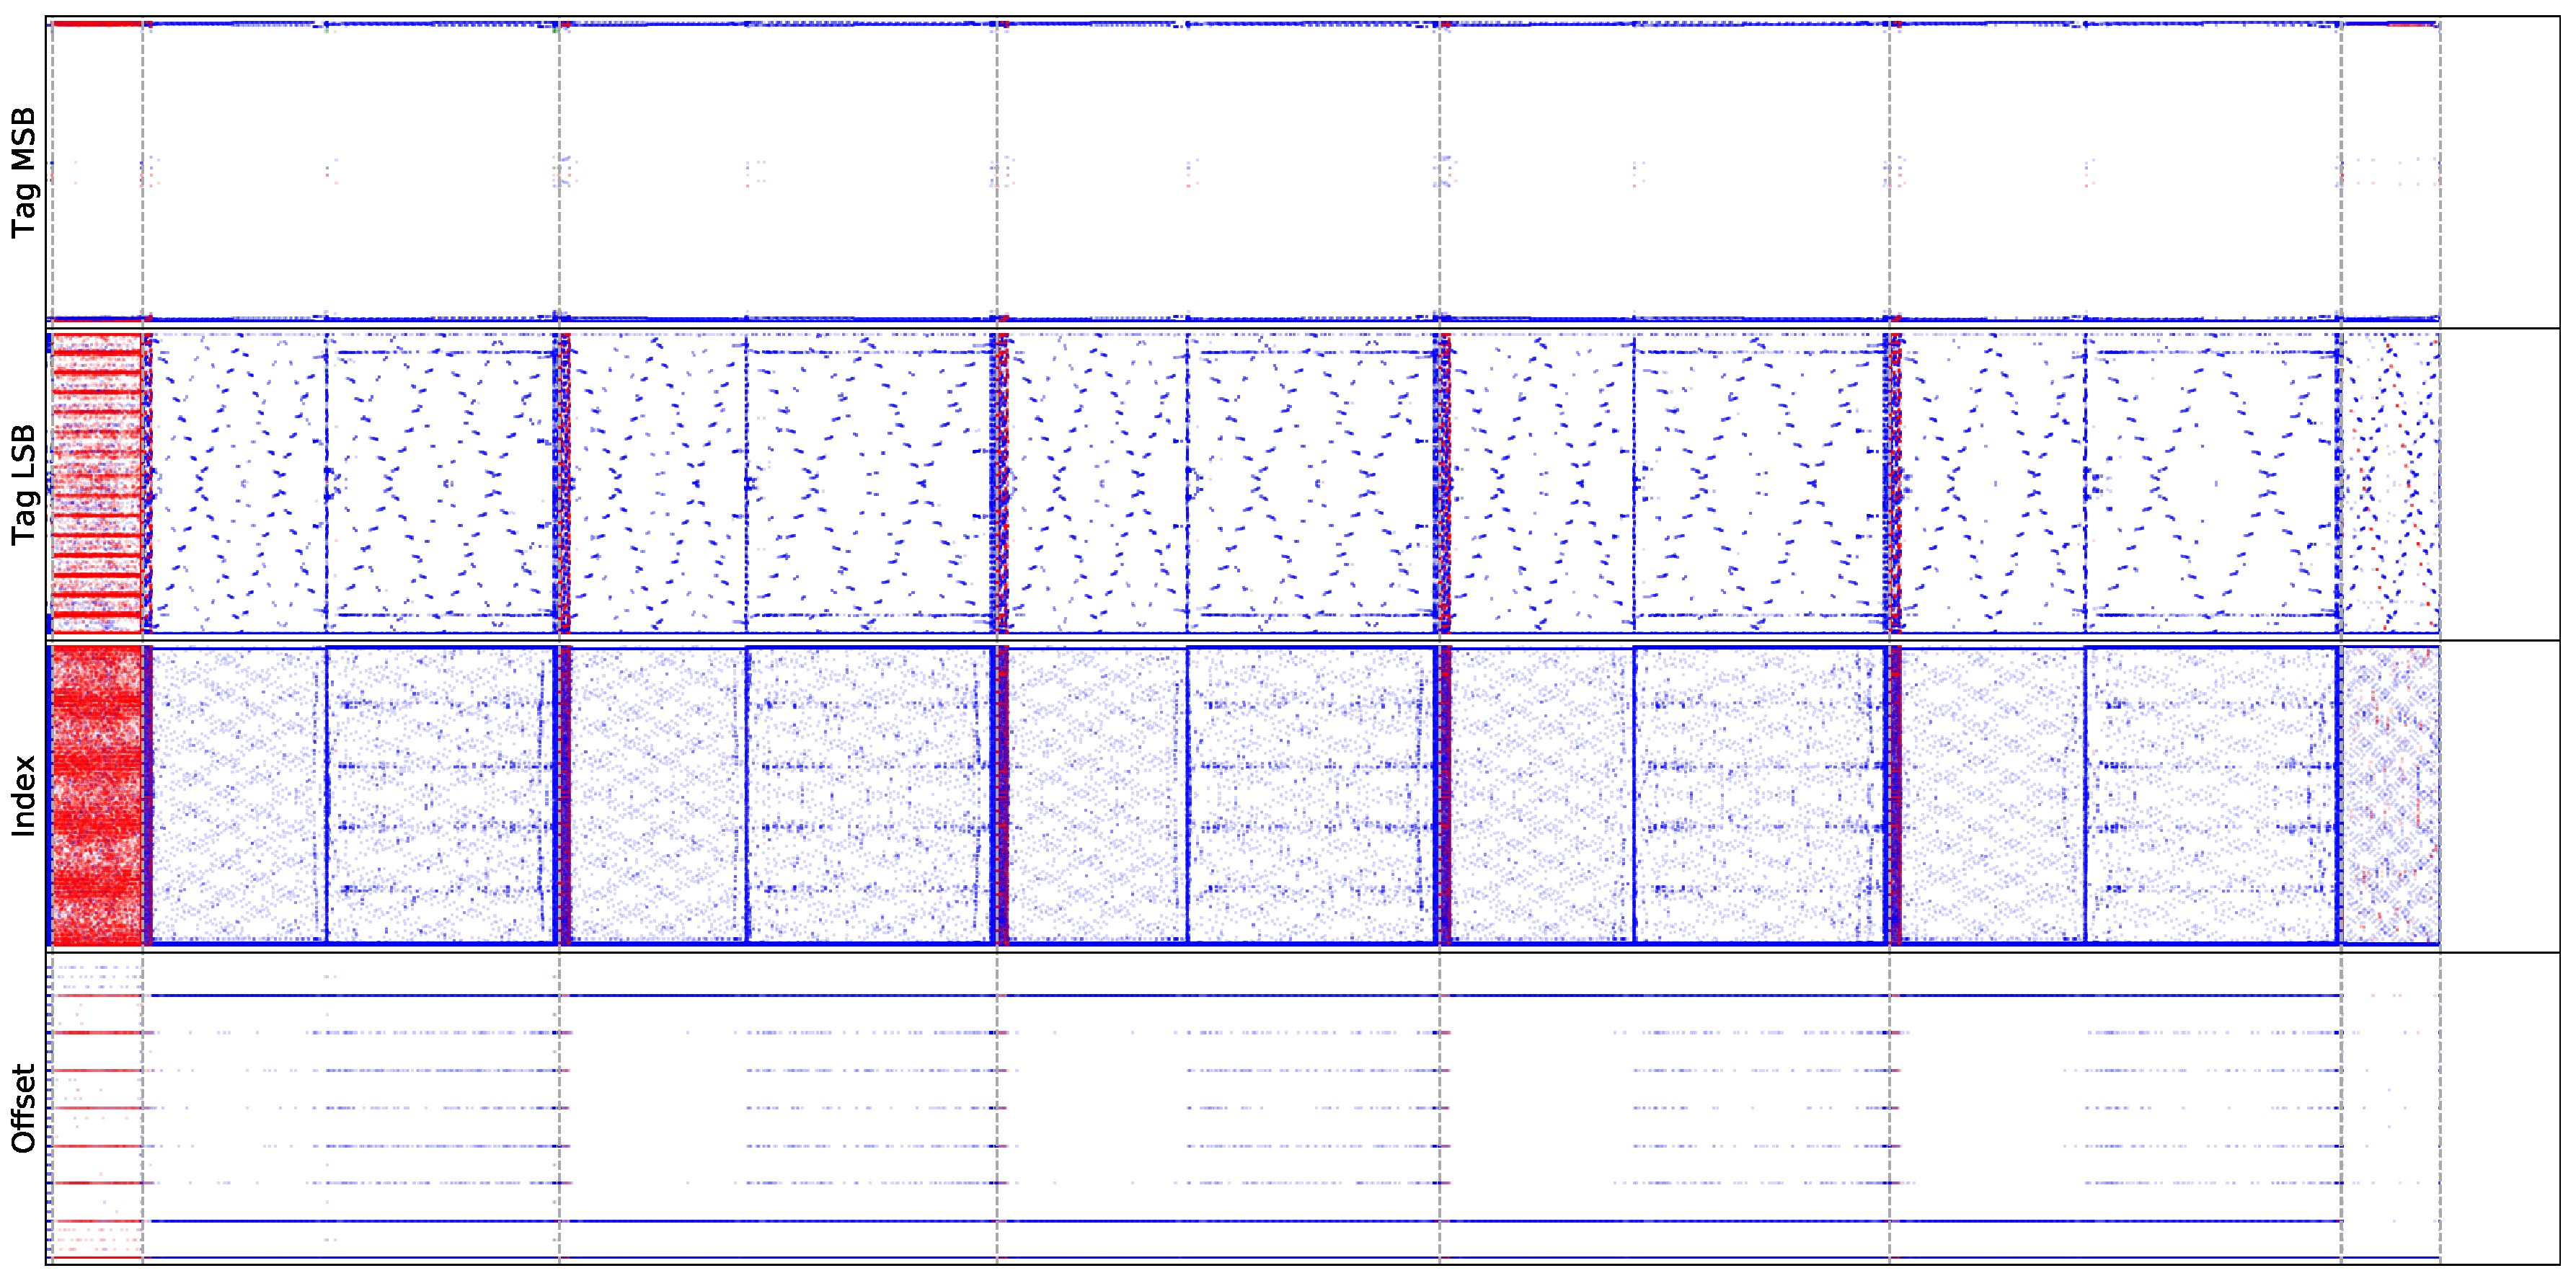
\includegraphics[width=\linewidth]{graphics/figures/src/fluidanimate-small.pdf}
		\caption{\label{fig:fluidanimate-small}\texttt{fluidanimate-small.pdf}}
	\end{subfigure}
	\begin{subfigure}[t]{\linewidth}
		\centering
		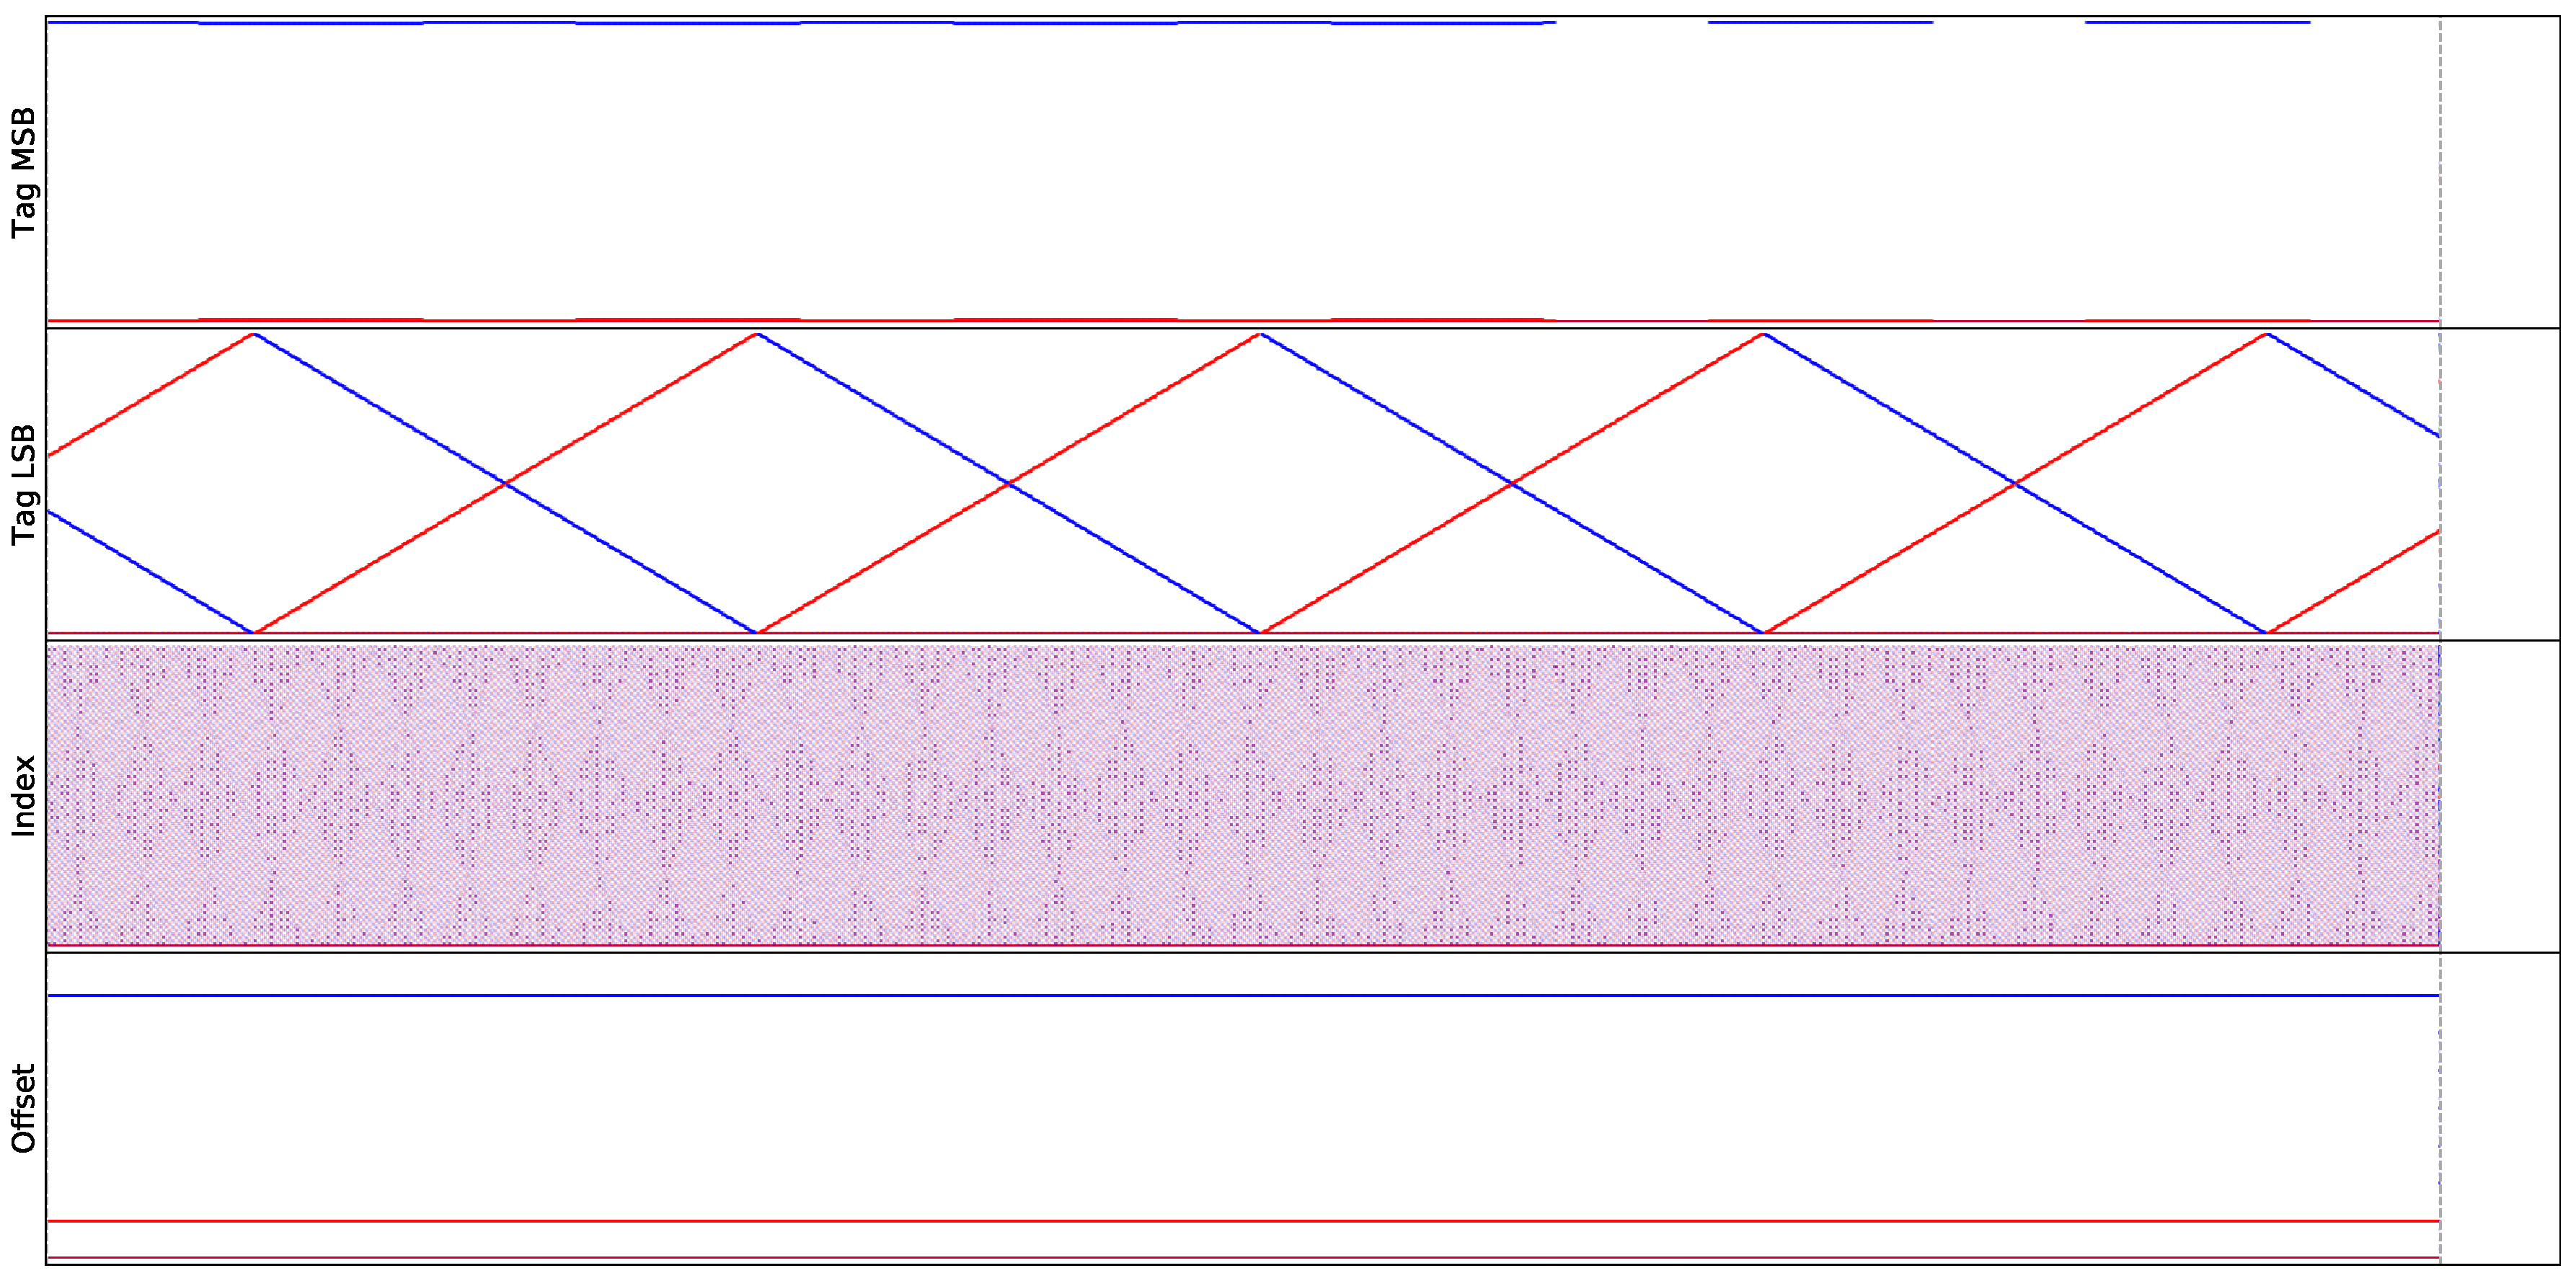
\includegraphics[width=\linewidth]{graphics/figures/adpcm-d-large.pdf}
		\caption{\label{fig:adpcm}\texttt{adpcm-d-small.pdf}}
	\end{subfigure}
	\caption{\label{fig:nb-phases}Exemples de découpage d'applications de l'ensemble de validation}
\end{figure}

\newcommand{\nothing}{-}
\begin{table}[h!]
\renewcommand{\arraystretch}{1.3}
	\begin{tabular}{l l l c c c}
\toprule
& & & \multicolumn{3}{c}{Nombre de points} \\
Suite & Benchmark & Description & \texttt{small} & \texttt{medium} & \texttt{large} \\
\midrule
%adpcm-c-large           & 1 \\
%adpcm-d-small           & 1 \\
\multirow{7}{*}{\textsc{PARSEC}} & blackscholes & Application financière & 1 & 1 & 1 \\
%blackscholes-medium     & 1 \\
%blackscholes-small      & 1 \\
& \texttt{bodydtrack} & Tracking vidéo & 3 & 6 & 12 \\
% bodytrack-large         & 12 \\
% bodytrack-medium        & 6 \\
% bodytrack-small         & 3 \\
& \texttt{canneal} & Optimisation & 1 & 1 & \nothing \\
% canneal-medium          & 1 \\
% canneal-small           & 1 \\
% fft-medium              & 3 \\
% fft-small               & 2 \\
& \texttt{fluidanimate} & Simulation de fluide & 5 & 5 & 5 \\
% fluidanimate-large      & 5 \\
% fluidanimate-medium     & 5 \\
% fluidanimate-small      & 5 \\
& \texttt{freqmine} & Fouille de donnée & 6 & 6 & 6 \\
% freqmine-large          & 6 \\
% freqmine-medium         & 6 \\
% freqmine-small          & 6 \\
% patricia-large          & 1 \\
% patricia-small          & 1 \\
% qsort-large             & 1 \\
% rijndael-enc-large      & 1 \\
% rijndael-enc-small      & 1 \\
% sha-large               & 1 \\
% sha-small               & 1 \\
& streamcluster & Clustering & 3 & \nothing & \nothing \\
% streamcluster-small     & 3 \\
& swaptions & Application financière & 1 & 1 & \nothing \\
% swaptions-medium        & 1 \\
% swaptions-small         & 1 \\
\midrule
\multirow{8}{*}{\textsc{MiBench}} & adpcm-c & Encodage audio & 1 & \nothing & 1 \\
& adpcm-d & Décodage audio & 1 & \nothing & 1\\
& fft & Transformée de Fourrier rapide & 2 & 3 & \nothing \\
& patricia & & 1 & \nothing & 1 \\
& qsort & Tri & \nothing & \nothing & 1 \\
& rijndael-dec & Chiffrement & 1 & \nothing & 1 \\
% rijndael-dec-large      & 1 \\ 
% rijndael-dec-small      & 1 \\
& rijndael-enc & Chiffrement & 1 & \nothing & 1 \\
& sha & Hachage & 1 & \nothing & 1 \\
\bottomrule
\end{tabular}
\caption{\label{table:appli-validation}Applications de l'ensemble de validation}
\end{table}

\subsection{Ensemble de caractéristiques}

Notre évaluation porte sur la pertinence de tel ou telle caractéristique de l'activité mémoire en isolation pour prédire le surcoût temporel induit par les interférences sur le système mémoire.
Nous considérons les caractéristiques présentées dans le chapitre précédent et résumées dans le tableau~\ref{table:feature_description}.

\begin{table}
\centering
	\renewcommand{\arraystretch}{1.3}
	%\setlength{\tabcolsep}{11pt}

\begin{tabular}{l l l l l}
	\toprule
    %							  &  				  					  &  				& \multicolumn{2}{c}{\textbf{Défini}}  \\
    \textbf{Caractéristique} 	  & \textbf{Description} 				  & \textbf{Source} & \textbf{Page} & \textbf{Section} \\
	\midrule
	 $BW_{iso}^{DDR}$ & Bande Passante (DRAM) 				  		& M  & \pageref{subsection:quantitative} & \ref{subsection:quantitative} \\
	 $BW_{iso}^{L2}$  & Bande passante (Cache L2) 			  		& C  & \pageref{subsection:quantitative}& \ref{subsection:quantitative} \\
	 $RW$ 			  & Taux de lecture / écritures 		  		& M  & \pageref{subsection:rw} & \ref{subsection:rw} \\
	 $DBI$ 			  & Inversion du bus de données par accès 		& V  & \pageref{subsection:dbi} & \ref{subsection:dbi} \\
	 $\overline{H}$   & Entropie normalisée des accès (bits [0,31]) & V  & \pageref{subsection:entropie} & \ref{subsection:entropie} \\
	 $H_{offset}$ 	  & Entropie des accès (bits [0,4])	 	  		& V  & \pageref{subsection:entropie}& \ref{subsection:entropie} \\
	 $H_{index}$  	  & Entropie des accès (bits [5, 15])  	  		& V  & \pageref{subsection:entropie} & \ref{subsection:entropie}\\
	 $H_{tagLSB}$ 	  & Entropie des accès (bits [16, 23]) 	  		& V  & \pageref{subsection:entropie} & \ref{subsection:entropie}\\
	 $H_{tagMSB}$ 	  & Entropie des accès (bits [24, 31]) 	  		& V  & \pageref{subsection:entropie} & \ref{subsection:entropie}\\
     $\tau$  		  & Impact du temps de service 			  		& MC & \pageref{subsection:tau} & \ref{subsection:tau}\\
	\bottomrule
\end{tabular}
\caption{\label{table:feature_description}Caractéristiques évaluées}
\end{table}

Afin de limiter le nombre de tests, nous regroupons ces caractéristiques dans différents ensembles, résumés dans le tableau~\ref{table:feature-sets}.
Ces ensembles peuvent être divisés en trois catégories:
\begin{itemize}
	\item Le groupe des \emph{caractéristiques quantitatives} regroupe les ensembles contenant les différentes bandes passantes,
	\item Le groupe des \emph{métriques qualitatives} regroupe les métriques ayant un rapport avec les types de requêtes effectuées ou encore la complexité des séquences d'accès.
	\item Le facteur $\tau$~(défini en section \ref{subsection:tau}) est une mesure de l'impact du temps de service des accès DRAM sur la vitesse de progression de l'application.
	Ce que ce facteur mesure étant différent des autres métriques qualitatives, nous avons choisi de l'isoler dans sa propre catégorie.

	% \item Nous avons fait le choix d'isoler le facteur $\tau$ dans sa propre catégorie, car celui ci mesure quelque chose de différents par rapport aux métriques du groupe quantitatif et qualitatif.
	% En effet le facteur $\tau$ ne quantifie pas des aspects liés à la sollicitation ou bien à la dégradation du temps de service des accès mémoire, mais à la propagation de ces dégradations de temps de service dans le temps d'exécution final.
\end{itemize}

\begin{table}
	\centering
	\setlength{\tabcolsep}{22pt}
	\begin{tabular}{l l l}
		\toprule
		\textbf{Nom} & \textbf{Définition} & \textbf{Groupe} \\
		\midrule
	 		$B^{DRAM}$ & $\{BW_{iso}^{DRAM}\}$ & \multirow{3}{*}{Quantitatif}\\
	 		$B^{L2}$ & $\{BW_{iso}^{L2}\}$ & \\
	 		$B$ & $B^{DRAM} \cup B^{L2}$ & \\
		\midrule
		$RW$ & $\{RW, DBI\}$ & \multirow{3}{*}{Qualitatif} \\
		$H$  & $\{\overline{H},H_{offset},H_{index},H_{tagLSB},H_{tagMSB}\}$ & \\
		$Q$ & $RW \cup H$ \\
		\midrule
		$\tau$ & $\{\tau\}$  & $\tau$ \\
		\bottomrule
	\end{tabular}
	\caption{\label{table:feature-sets}Ensembles de caractéristiques évaluées}
\end{table}

Notre évaluation portera donc sur les trois ensembles du groupe quantitatif.
Pour chacun de ces ensembles, nous évaluerons le gain apporté par les métriques qualitatives (en ajoutant l'ensemble $Q$) seules et en conjonction avec $\tau$.

\subsection{Résultats}

L'évaluation porte sur la précision que l'on peut atteindre pour l'inférence de surcoût temporelle en fonction des caractéristiques que l'on prend en entrée.
Nos expériences portent sur trois points:
\begin{itemize}
	\item L'impact de la caractérisation quantitative employée.
	\item Le gain éventuel apporté par les caractéristiques qualitatives.
	\item Le gain éventuel apporté par le facteur $\tau$.
\end{itemize}

Nous mesurons la qualité de la prédiction  à l'aide de deux métriques : l'erreur quadratique moyenne (ou MSE pour Mean Squared Error) et l'erreur absolue moyenne (ou MAE pour Mean Absolute Error) de l'ensemble de validation.
Si $M$ désigne un ensemble de points à évaluer, alors ces deux métriques sont définies ainsi:

\begin{equation}
	\label{equation:mse}
	MSE(M) = \frac{1}{|M|} \sum_{m\in M} (predicted(m) - observed(m))^2
\end{equation}

\begin{equation}
	\label{equation:mae}
	MAE(M) = \frac{1}{|M|} \sum_{m\in M} |predicted(m) - observed(m)|
\end{equation}

Ces deux métriques ont deux rôles différents.
La MAE donne une mesure directement interprétable de l'erreur observée pour l'ensemble de validation.
La MSE est utilisée pour déterminer l'ampleur des erreurs de prédictions sur l'ensemble de validation.
En effet, cette métrique donne un poids plus important aux applications proportionnellement à l'erreur observée.
Elle pénalise donc les ensembles de caractéristiques entrainant des erreurs de mesures conséquentes, même si ces dernières ne concernent qu'un nombre réduit de points.
La fonction $predicted$ donne le plus grand surcoût temporel observé pour une application, celui-ci étant déterminé à l'aide du protocole défini dans la section~\ref{section:protocole}.

% We consider the combinations of three sets of features we named $B$, $Q$, and $\tau$.
% $B$ and $\tau$ are singletons comprising respectively the bandwidth in isolation and the impact factor defined in Section~\ref{section:qualitative}.
% $Q$ is a set of qualitative features presented in Section~\ref{section:qualitative}.
% It comprises the read over write ratio, the interleaving rate of read and write accesses, the pattern entropy and the split address.
% The address is split in four parts: offset (bits $[0,5[$), index (bits $[5,16[$), tag's lower half (bits $[16, 24[$), and tag's upper half (bits $[24, 32[$).
% We present the results for three combinations of features: $B$, $BQ$ and $BQ\tau$. 
% $B$ is the baseline, $BQ$ and $BQ\tau$ are meant to evaluate respectively the relevance of qualitative metrics and the impact factor $\tau$.

% We measure the quality of prediction of the validation set with the \emph{Mean Squared Error (MSE)} and the \emph{Mean Absolute error (MAE)}.
% The base of comparison is the worst overhead measured using the protocol described in Section~\ref{section:protocole}.
% The MSE gives a higher penalty to important mispredictions; hence this metric is useful to evaluate the range of mispredictions.
% Whereas, the MAE gives the average prediction error encountered on the dataset.

La figure~\ref{fig:prediction_error} illustre le résultat de l'inférence pour les différents ensembles de caractéristiques que nous évaluons.
Plus le nuage de points rouge y est resserré plus l'inférence est précise.
Notons tout d'abord l'importance du choix de la caractérisation quantitative.
Prises seules $BW^{DRAM}_{iso}$ et $BW^{L2}_{iso}$ se révèlent très imprécises, ce qui n'est pas étonnant au vu de la dispersion observée dans le chapitre précédent.
Ce résultat illustre le manque de précision intrinsèque aux approches de régulations basées l'inspection d'une seule ressource.
Par contre, un gain substantiel est observable lorsque l'on combine ces deux bandes passantes (respectivement 92,6\% et 76,5\% de réduction d'erreur quadratique moyenne par rapport à $BW^{L2}$ et $BW^{DRAM}$).

\begin{figure}[h!]
	\begin{tabular}{c c c}
	\begin{subfigure}[t]{0,31\linewidth}
		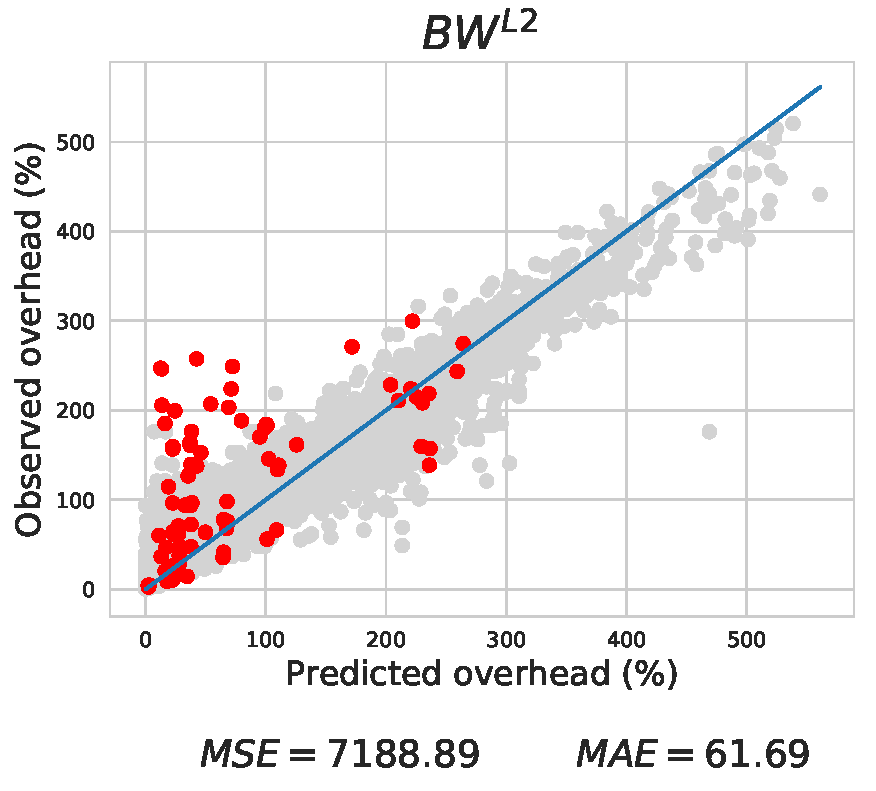
\includegraphics[width=\textwidth]{figures/L1.pdf}
		%\caption{\label{fig:pred_b}$b$}
	\end{subfigure} & 
	\begin{subfigure}[t]{0,31\linewidth}
		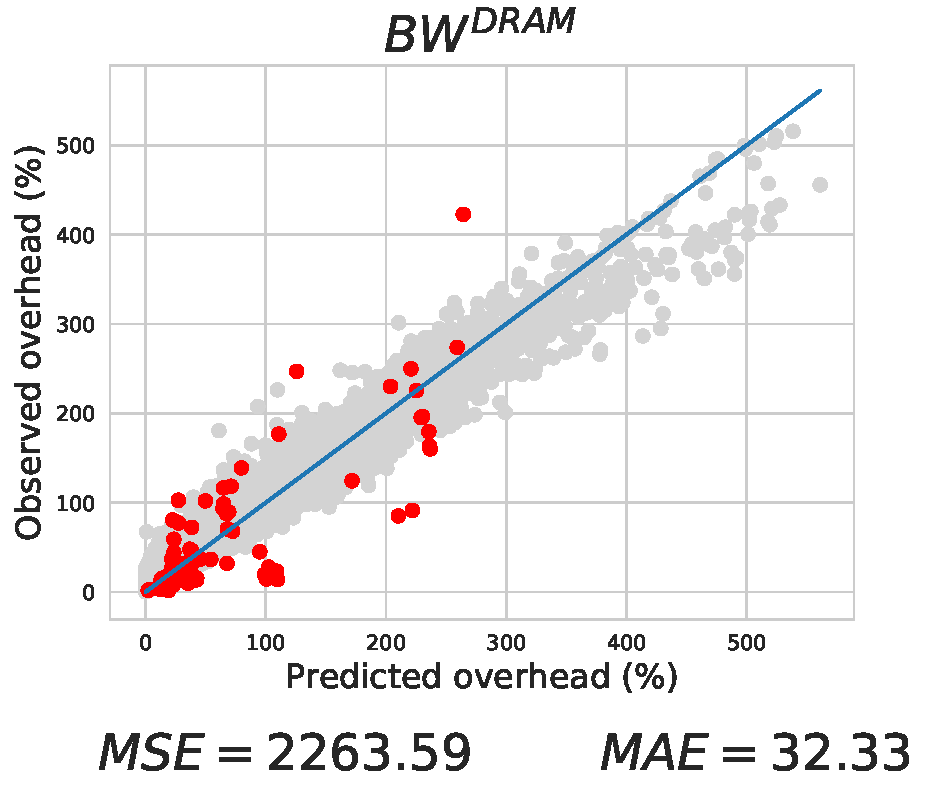
\includegraphics[width=\textwidth]{figures/b.pdf}
		%\caption{\label{fig:pred_b}$b$}
	\end{subfigure} & 
	\begin{subfigure}[t]{0,31\linewidth}
		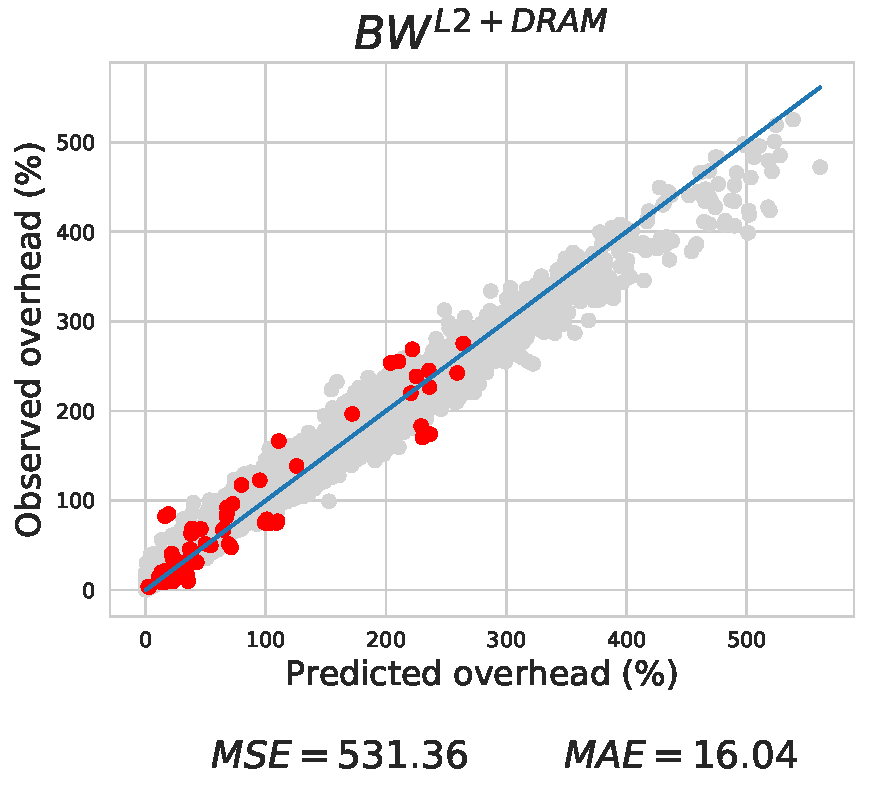
\includegraphics[width=\textwidth]{figures/B.pdf}
		%\caption{\label{fig:pred_b}$b$}
	\end{subfigure}\\
	\par\bigskip

	\begin{subfigure}[t]{0,31\linewidth}
		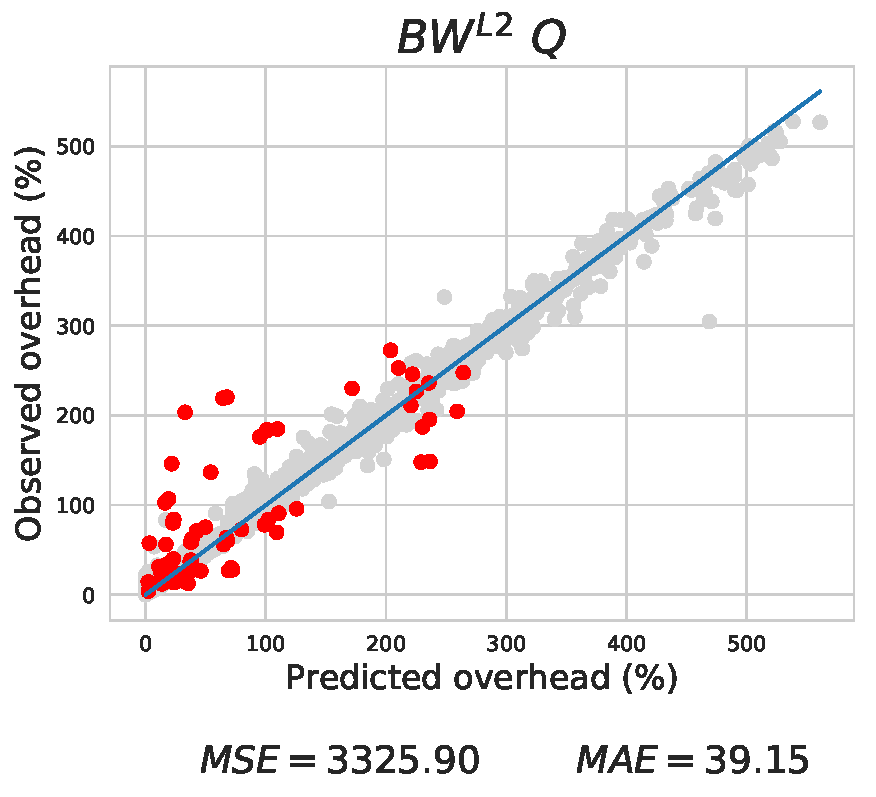
\includegraphics[width=\textwidth]{figures/L1_Q.pdf}
		%\caption{\label{fig:pred_b}$b$}
	\end{subfigure} & 
	\begin{subfigure}[t]{0,31\linewidth}
		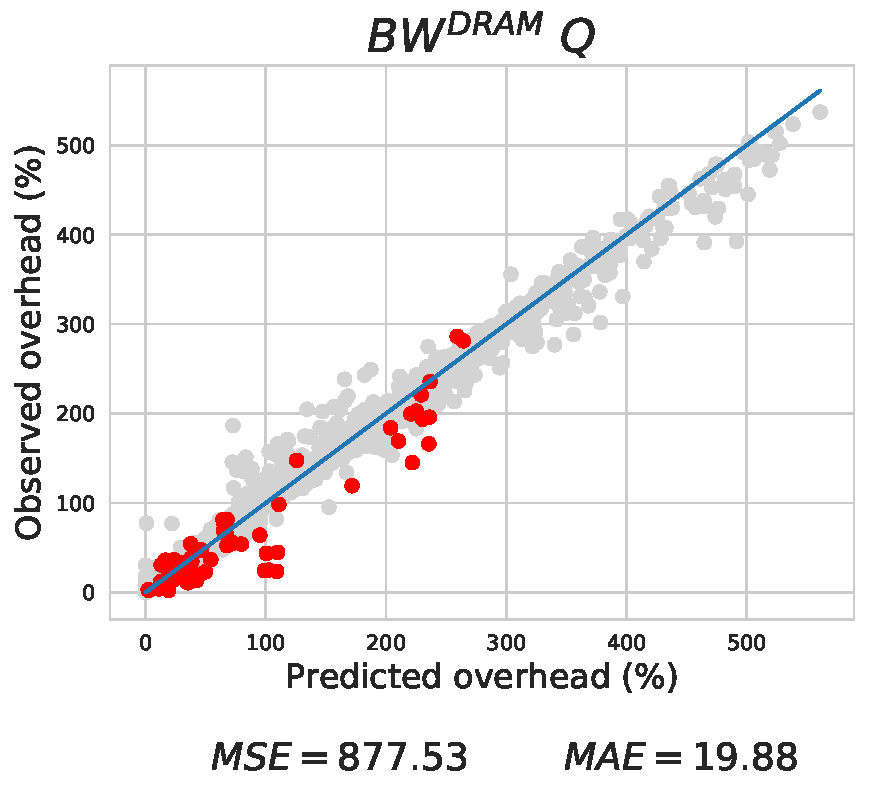
\includegraphics[width=\textwidth]{figures/b_Q.pdf}
		%\caption{\label{fig:pred_b}$b$}
	\end{subfigure} &
	\begin{subfigure}[t]{0.31\linewidth}
		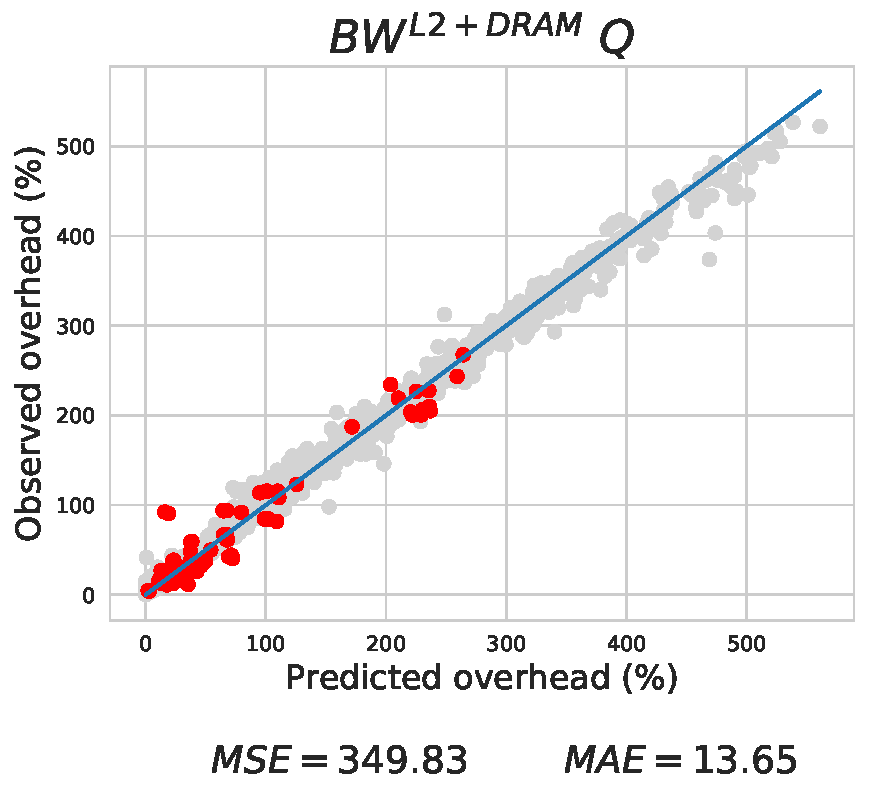
\includegraphics[width=\textwidth]{figures/B_Q.pdf}
		%\caption{\label{fig:pred_b}$b$}
	\end{subfigure} \\
	\par\bigskip

	\begin{subfigure}[t]{0,31\linewidth}
		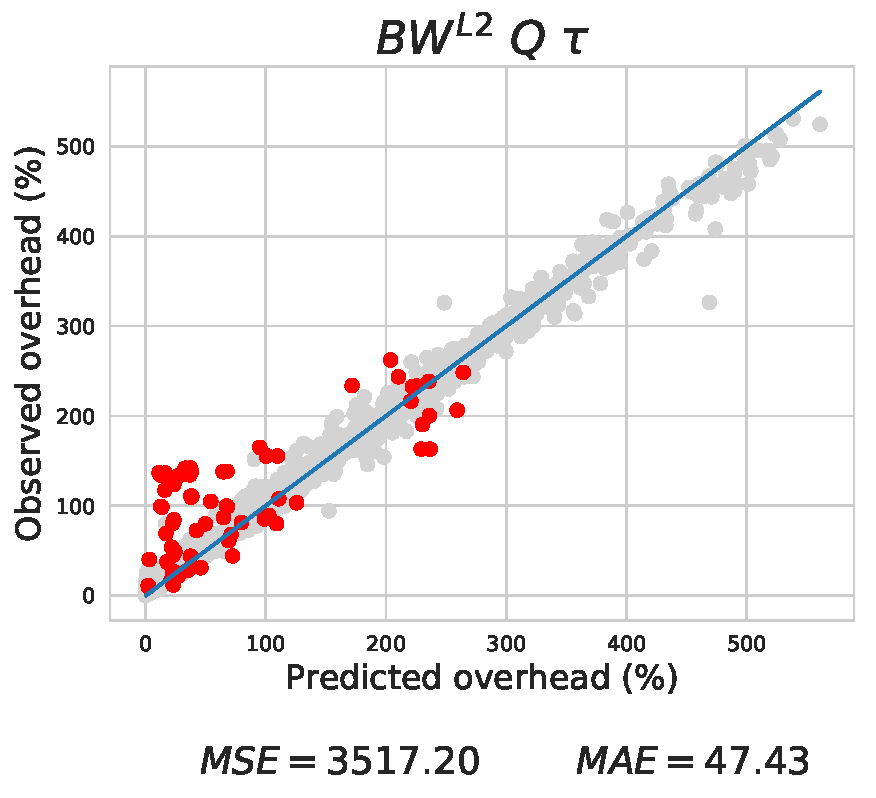
\includegraphics[width=\textwidth]{figures/L1_Q_tau.pdf}
		%\caption{\label{fig:pred_b}$b$}
	\end{subfigure} &
	\begin{subfigure}[t]{0,31\linewidth}
		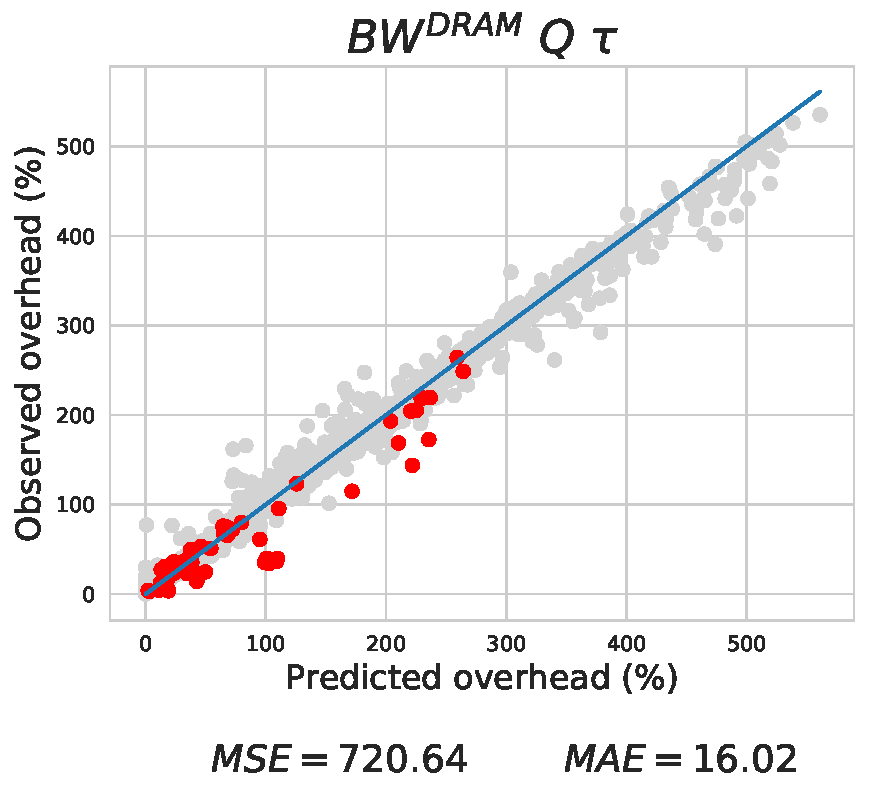
\includegraphics[width=\textwidth]{figures/b_Q_tau.pdf}
		%\caption{\label{fig:pred_b}$b$}
	\end{subfigure} &
	\begin{subfigure}[t]{0,31\linewidth}
		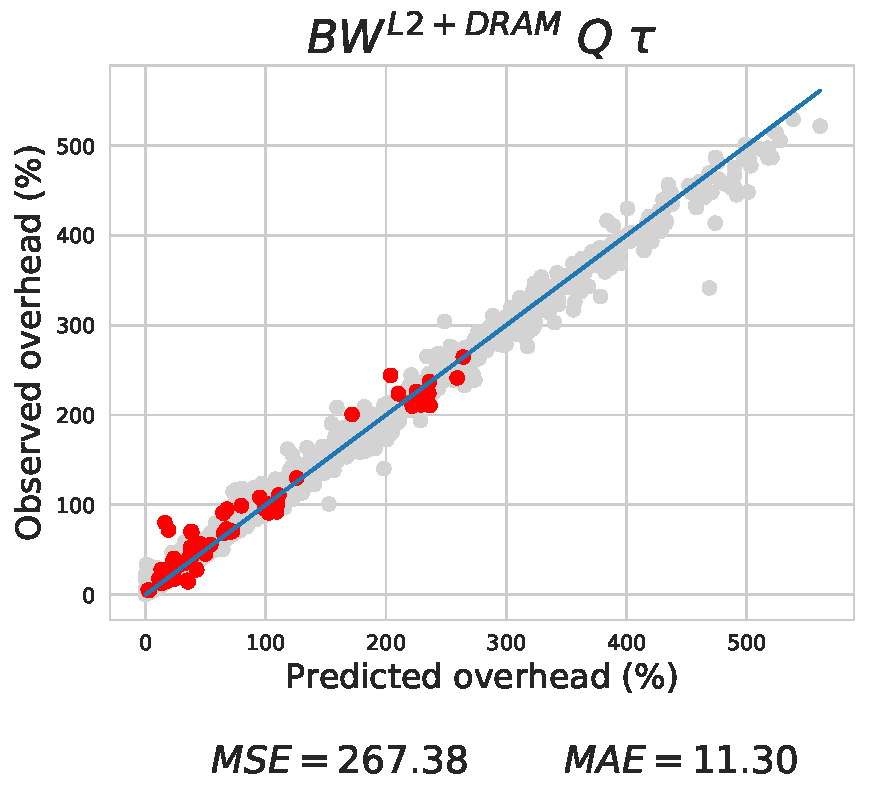
\includegraphics[width=\textwidth]{figures/B_Q_tau.pdf}
		%\caption{\label{fig:pred_b}$b$}
	\end{subfigure} \\
	\end{tabular}
	\par\bigskip
	
	\caption{\label{fig:prediction_error}Valeurs prédites en fonction des valeurs observées. Les points gris correspondent aux applications de l'ensemble d'entrainement, tandis que les points rouges correspondent aux applications de l'ensemble de validation.} 
\end{figure}

La deuxième observation porte sur l'apport du groupe de caractéristiques qualitatives pour l'inférence de surcoût temporel.
L'ajout de métriques qualitatives permet d'améliorer significativement la qualité de prédiction, et ce quelque soit le groupe de métrique quantitative employée. La réduction d'erreur de prédiction est résumée dans le tableau suivant.

\begin{table}[h!]
\centering
\renewcommand{\arraystretch}{1.3}
\begin{tabular}{l l l l}
	\toprule
\textbf{Ensemble quantitatif}	& $BW_{iso}^{L2}$ & $BW_{iso}^{DRAM}$ & $BW_{iso}^{L2 + DRAM}$ \\
	\midrule
\textbf{Réduction de MSE}		&      	  55,1\%  &       	   61,2\% &       			34,2\% \\
\textbf{Réduction de MAE}		&       36,5\%      &       38,5\% 	  &         16,2\%            \\
	\bottomrule
\end{tabular}
\caption{\label{table:gain-qualitatif}Gain de performance de prédiction apporté par les métriques qualitatives}
\end{table}

En moyenne le gain apporté par le facteur $\tau$ est relativement modeste, il permet néanmoins d'obtenir la meilleure prédiction.
Si on utilise l'ensemble $BW_{iso}^{L2}$ comme caractérisation quantitative, la qualité de prédiction est en moyenne légèrement dégradée.
L'examen des erreurs de prédictions maximales (tableau~\ref{table:max-error}) révèle néanmoins un gain que ce soit en sur ou en sous-estimation.


\begin{table}
	\centering
	\renewcommand{\arraystretch}{1.3}
	\begin{tabular}{r c c c c}
	\toprule
	Quantitatif  & $Q$ & $\tau$ & Sous-estimation & Surestimation \\
	\midrule
\multirow{3}{*}{$BW_{iso}^{L2}$} 	   	&   &    & 97,47 & 234,45 \\
										& x &    & 88,11 & 170,69 \\
 										& x & x  & 73.72 & 125.47 \\
\midrule
\multirow{3}{*}{$BW_{iso}^{DRAM}$} 	   	&   &    & 130,64 & 158,43 \\
     								   	& x &    & 85,50  & 27,16 \\
   									   	& x & x  & 78.15  & 14.76 \\
\midrule
\multirow{3}{*}{$BW_{iso}^{L2 + DRAM}$} &   &    & 62,74 & 66,39 \\
 										& x &    & 31,78 & 76,21 \\
										& x & x  & 26.16 & 63.81 \\
\bottomrule
	\end{tabular}
	\caption{\label{table:max-error}Plus grande sur et sous-estimation observée pour l'ensemble de validation (valeurs absolues)}
\end{table}

\section{Conclusions}

Dans ce chapitre, nous avons utilisé les données issues de nos microbenchmarks pour capturer le comportement du matériel concernant les interférences.
Cette étude nous a permis d'évaluer la pertinence de deux de nos outils pour l'apprentissage automatique de ce comportement :
% Dans ce chapitre, nous avons montré comment utilisé les outils et métriques présentées dans cette thèse pour prédire le surcoût temporel subi par une application à cause des interférences.
% Nous avons notamment évaluer la pertinence de différentes combinaisons de métriques caractérisant les comportements applicatifs en isolation pour l'inférence du surcoût temporel induit par les interférences.
% Cette évaluation repose sur des techniques d'apprentissages automatiques.
% Elle montre l'impact de deux outils que nous avons présenté dans cette thèse :
\begin{itemize}
	\item Nos \emph{microbenchmarks} sont utilisés pour l'entrainement de la fonction de prédiction.
	On évalue donc si la couverture de comportements qu'ils offrent est suffisante pour permettre à la fonction de prédiction de capturer efficacement le comportement du matériel.
	\item Nos \emph{différentes métriques} sont utilisées pour la caractérisation du comportement.
	L'évaluation porte donc également sur la pertinence de l'information qu'elles apportent sur la sensibilité au problème d'interférences.
\end{itemize}

Les résultats de cette étude montrent plusieurs choses.
Tout d'abord, l'utilisation d'une seule caractéristique quantitative ne donne pas de bons résultats.
On observe des gains significatifs de précision en prenant en compte les différentes bandes passantes que l'on peut mesurer.
Ensuite, on note que l'ajout de métriques qualitatives permet toujours d'améliorer la précision de la prédiction et ceux quelque soit l'ensemble de métriques quantitatives auxquels elles sont associées.
De plus, on note une forte réduction dans la sous-estimation du surcoût, ce qui s'avère appréciable dans un contexte temps-réel.
L'ajout du facteur $\tau$, permet un gain supplémentaire de précision.
Enfin, on peut noter que nos microbenchmarks permettent de capturer assez efficacement le comportement du matériel.
En effet, pour l'ensemble de caractéristiques donnant les meilleurs résultats, l'erreur de prédiction absolue  observée en moyenne sur l'ensemble de validation est de 11,3\%, la plus forte sous-estimation étant d'environ 23\%.

Ce chapitre clôt la présentation des différentes contributions de cette thèse.
Dans le chapitre suivant, nous allons conclure ce document, et également présenter les différentes perspectives qui s'offrent à nous pour étendre ces travaux.

% The prediction error per application and for the whole validation set is summarized in the Table~\ref{table:results_nc}.
% There is a clear improvement of prediction precision from the baseline for the $BQ$ and the $BQ\tau$ sets.
% This indicates the relevance of the metrics in the $Q$ and the $\tau$ sets to characterize interference sensitivity, but also that our microbenchmarks offer 
% a good coverage of memory consumption nature and intensity.
% The greatest improvements are observed for \texttt{streamcluster-small}, \texttt{canneal-small}, and \texttt{canneal-medium}.
% The effect of the $\tau$ impact factor is clearly more important on the MSE than on the MAE, indicating that it reduces the range of mispredictions.
% The gain of accuracy brought by the $Q$ and the $\tau$ sets is observable on the Figure~\ref{fig:prediction_error} showing the predicted and the observed values of each test case.
% i
% \begin{table}[!h]$$
% 	\renewcommand{\arraystretch}{1.2}
% 	\caption{\label{table:results_nc}Mean squared and absolute prediction error (MSE and MAE) per application and for the whole validation set}
% 	\resizebox{\columnwidth}{!}{%
% 		\rowcolors{2}{gray!15}{}
% \begin{tabular}{l l l l l l l}
% 	\toprule
% 	& $b$ & $b Q$ & $b Q \tau$ & $B$ & $B Q$ & $B Q \tau$ \\
% 	\midrule
% 	adpcm-c-large  & 	7.82 & 	56.48 & 	0.06& 	2.25 &  	50.09 & 	0.02 \\
% 	adpcm-c-small  & 	51.16 & 	54.37 & 	20.37& 	5.28 &  	20.35 & 	93.26 \\
% 	adpcm-d-large  & 	247.88 & 	1.80 & 	63.83& 	376.70 &  	10.93 & 	67.62 \\
% 	adpcm-d-small  & 	25.12 & 	1.56 & 	65.37& 	374.67 &  	10.45 & 	69.26 \\
% 	blackscholes-large  & 	47.59 & 	451.84 & 	313.76& 	12.97 &  	84.42 & 	179.75 \\
% 	blackscholes-medium  & 	97.52 & 	406.12 & 	270.05& 	73.66 &  	184.37 & 	249.22 \\
% 	blackscholes-small  & 	66.25 & 	53.95 & 	44.90& 	19.91 &  	25.90 & 	35.56 \\
% 	bodytrack-large  & 	2934.93 & 	1365.09 & 	1357.57& 	350.18 &  	214.89 & 	113.96 \\
% 	bodytrack-medium  & 	2882.84 & 	1704.28 & 	1558.25& 	302.03 &  	272.96 & 	201.44 \\
% 	bodytrack-small  & 	3388.90 & 	2562.92 & 	1948.82& 	408.76 &  	706.91 & 	504.02 \\
% 	canneal-medium  & 	6058.59 & 	1349.28 & 	260.32& 	139.11 &  	676.86 & 	26.66 \\
% 	canneal-small  & 	1565.97 & 	1122.48 & 	121.77& 	2792.13 &  	634.00 & 	74.44 \\
% 	fft-large  & 	3986.99 & 	379.81 & 	11.27& 	98.04 &  	63.67 & 	147.96 \\
% 	fft-medium  & 	8481.46 & 	137.90 & 	165.91& 	1074.94 &  	5.16 & 	19.64 \\
% 	fft-small  & 	1680.93 & 	324.26 & 	1.46& 	564.54 &  	38.49 & 	129.36 \\
% 	fluidanimate-large  & 	37.41 & 	191.01 & 	79.94 & 	65.86 &  	64.62 & 	80.91 \\
% 	fluidanimate-medium  & 	265.46 & 	27.51 & 	12.94 & 	735.86 &  	457.30 & 	763.45 \\
% 	fluidanimate-small  & 	1596.67 & 	107.45 & 	2.43 & 	8.52 &  	39.56 & 	86.89 \\
% 	freqmine-large  & 	4041.76 & 	1817.21 & 	1762.44 & 	553.23 &  	233.39 & 	84.84 \\
% 	freqmine-medium  & 	2913.38 & 	516.09 & 	507.50 & 	445.56 &  	226.89 & 	76.52 \\
% 	freqmine-small  & 	1158.56 & 	453.19 & 	371.55 & 	591.98 &  	544.71 & 	322.00 \\
% 	patricia-large  & 	396.95 & 	524.05 & 	147.51 & 	331.76 &  	448.16 & 	305.41 \\
% 	patricia-small  & 	620.82 & 	587.52 & 	170.67 & 	613.61 &  	555.25 & 	403.22 \\
% 	qsort-large  & 	2313.25 & 	2752.08 & 	2806.46 & 	712.30 &  	617.48 & 	843.84 \\
% 	rijndael-dec-large  & 	17.66 & 	6.74 & 	7.83 & 	14.14 &  	11.14 & 	1.00 \\
% 	rijndael-dec-small  & 	1.23 & 	15.24 & 	37.56 & 	46.70 &  	35.26 & 	0.72 \\
% 	rijndael-enc-large  & 	73.96 & 	26.95 & 	7.56 & 	76.38 &  	39.41 & 	5.97 \\
% 	rijndael-enc-small  & 	252.69 & 	76.72 & 	3.34 & 	174.85 &  	111.17 & 	40.55 \\
% 	sha-large  & 	100.46 & 	100.71 & 	134.75 & 	114.80 &  	28.63 & 	1.24 \\
% 	sha-small  & 	5.19 & 	12.17 & 	28.00& 	40.34 &  	2.61 & 	17.56 \\
% 	streamcluster-small  & 	2577.15 & 	5.45 & 	321.84 & 	2555.47 &  	915.72 & 	410.68 \\
% 	swaptions-medium  & 	0.50 & 	15.38 & 	15.69 & 	4187.30 &  	6262.42 & 	3860.31 \\
% 	swaptions-small  & 	309.33 & 	284.02 & 	228.44 & 	4182.90 &  	5028.70 & 	2489.72 \\
% \end{tabular}}
% \end{table}

% \begin{table}[!h]
% 	\renewcommand{\arraystretch}{1.2}
% 	\caption{\label{table:results_nc}Mean squared and absolute prediction error (MSE and MAE) per application and for the whole validation set}
% 	%\resizebox{\columnwidth}{!}{%
% 		\rowcolors{2}{gray!15}{}
% \begin{tabular}{l l l l l l l}
% 	\toprule
% 	& $b$ & $b Q$ & $b Q \tau$ & $B$ & $B Q$ & $B Q \tau$ \\
% 	\midrule
% 	adpcm-c-large  & 	2.80 & 	7.52 & 	0.25 & 	1.50 & 	7.08 & 	0.15 \\
% adpcm-c-small  & 	7.15 & 	7.37 & 	4.51 & 	2.30 & 	4.51 & 	9.66 \\
% adpcm-d-large  & 	15.74 & 	1.34 & 	7.99 & 	19.41 & 	3.31 & 	8.22 \\
% adpcm-d-small  & 	5.01 & 	1.25 & 	8.09 & 	19.36 & 	3.23 & 	8.32 \\
% blackscholes-large  & 	6.90 & 	21.26 & 	17.71 & 	3.60 & 	9.19 & 	13.41 \\
% blackscholes-medium  & 	9.88 & 	20.15 & 	16.43 & 	8.58 & 	13.58 & 	15.79 \\
% blackscholes-small  & 	8.14 & 	7.34 & 	6.70 & 	4.46 & 	5.09 & 	5.96 \\
% bodytrack-large  & 	44.49 & 	27.56 & 	23.48 & 	15.40 & 	11.93 & 	8.04 \\
% bodytrack-medium  & 	41.66 & 	29.80 & 	26.99 & 	11.78 & 	13.57 & 	12.00 \\
% bodytrack-small  & 	49.94 & 	37.77 & 	32.65 & 	13.52 & 	25.40 & 	21.90 \\
% canneal-medium  & 	77.84 & 	36.73 & 	16.13 & 	11.79 & 	26.02 & 	5.16 \\
% canneal-small  & 	39.57 & 	33.50 & 	11.04 & 	52.84 & 	25.18 & 	8.63 \\
% fft-large  & 	41.61 & 	16.00 & 	2.69 & 	8.09 & 	6.00 & 	8.28 \\
% fft-medium  & 	70.75 & 	9.58 & 	10.89 & 	22.52 & 	2.22 & 	3.47 \\
% fft-small  & 	29.09 & 	12.84 & 	1.21 & 	17.36 & 	5.13 & 	9.25 \\
% fluidanimate-large  & 	5.47 & 	10.85 & 	7.72 & 	7.12 & 	6.64 & 	8.29 \\
% fluidanimate-medium  & 	11.00 & 	5.24 & 	3.59 & 	27.07 & 	21.38 & 	27.63 \\
% fluidanimate-small  & 	26.21 & 	10.37 & 	1.20 & 	2.57 & 	6.28 & 	9.30 \\
% freqmine-large  & 	46.51 & 	29.95 & 	28.14 & 	14.87 & 	12.04 & 	6.91 \\
% freqmine-medium  & 	31.83 & 	19.37 & 	15.57 & 	16.35 & 	11.83 & 	5.79 \\
% freqmine-small  & 	27.53 & 	19.14 & 	15.28 & 	18.54 & 	19.67 & 	12.06 \\
% patricia-large  & 	19.92 & 	22.89 & 	12.15 & 	18.21 & 	21.17 & 	17.48 \\
% patricia-small  & 	24.92 & 	24.24 & 	13.06 & 	24.77 & 	23.56 & 	20.08 \\
% qsort-large  & 	48.10 & 	52.46 & 	52.98 & 	26.69 & 	24.85 & 	29.05 \\
% rijndael-dec-large  & 	4.20 & 	2.60 & 	2.80 & 	3.76 & 	3.34 & 	1.00 \\
% rijndael-dec-small  & 	1.11 & 	3.90 & 	6.13 & 	6.83 & 	5.94 & 	0.85 \\
% rijndael-enc-large  & 	8.60 & 	5.19 & 	2.75 & 	8.74 & 	6.28 & 	2.44 \\
% rijndael-enc-small  & 	15.90 & 	8.76 & 	1.83 & 	13.22 & 	10.54 & 	6.37 \\
% sha-large  & 	10.02 & 	10.04 & 	11.61 & 	10.71 & 	5.35 & 	1.11 \\
% sha-small  & 	2.28 & 	3.49 & 	5.29 & 	6.35 & 	1.61 & 	4.19 \\
% streamcluster-small  & 	41.16 & 	2.25 & 	16.27 & 	46.48 & 	27.70 & 	18.61 \\
% swaptions-medium  & 	0.70 & 	3.92 & 	3.96 & 	64.71 & 	79.14 & 	62.13 \\
% swaptions-small  & 	17.59 & 	16.85 & 	15.11 & 	64.68 & 	70.91 & 	49.90 \\
% \end{tabular}%}
% \end{table}

	% \begin{tabular}{r c c c c c c}
	% 	\toprule
	% 	\rowcolor{white}
	% 		Prediction error metric& \multicolumn{3}{c}{MAE} & \multicolumn{3}{c}{MSE}\\
	% 		%\cmidrule(lr){2-4}
	% 		%\cmidrule(lr){5-7}
	% 	\rowcolor{white}
	% 	\cmidrule(r){1-1}
	% 	\cmidrule(lr){2-4}
	% 	\cmidrule(l){5-7}
	% 	\rowcolor{white}
	% 	Application & $B$ & $BQ$ & $BQ\tau$ & $B$ & $BQ$ & $BQ\tau$ \\
	% 	\cmidrule(r){1-1}
	% 	\cmidrule(lr){2-4}
	% 	\cmidrule(l){5-7}
		
	% 	    adpcm-c-small & 32.4 & 2.6 & 16.6 & 1052.9 & 6.8 & 276.5 \\
    adpcm-c-large & 40.5 & 5.8 & 13.2 & 1638.2 & 33.7 & 174.0 \\
    adpcm-d-small & 65.3 & 6.1 & 19.8 & 4257.7 & 37.8 & 392.5 \\
    adpcm-d-large & 63.0 & 6.0 & 19.7 & 3970.5 & 36.6 & 388.6 \\
    blackscholes-small & 10.3 & 8.2 & 8.4 & 106.2 & 66.9 & 70.9 \\
    blackscholes-medium & 21.9 & 4.3 & 4.6 & 479.8 & 18.4 & 21.4 \\
    blackscholes-large & 28.4 & 1.2 & 4.5 & 804.1 & 1.5 & 19.9 \\
    bodytrack-small & 47.9 & 25.8 & 17.6 & 3103.3 & 1424.3 & 581.6 \\
    bodytrack-medium & 34.3 & 24.5 & 17.2 & 1546.4 & 1225.2 & 504.9 \\
    bodytrack-large & 25.9 & 22.5 & 15.2 & 837.1 & 1060.3 & 435.7 \\
    canneal-small & 141.0 & 16.5 & 25.9 & 19872.2 & 271.5 & 669.3 \\
    canneal-medium & 158.0 & 22.2 & 32.8 & 24966.0 & 493.8 & 1073.9 \\
    fft-small & 22.7 & 15.0 & 19.5 & 797.7 & 651.5 & 704.1 \\
    fft-medium & 29.0 & 18.0 & 16.8 & 1620.4 & 492.2 & 421.6 \\
    fft-large & 20.0 & 11.3 & 9.4 & 769.3 & 311.3 & 216.6 \\
    freqmine-small & 34.2 & 32.6 & 28.0 & 2056.1 & 1818.3 & 1344.1 \\
    freqmine-medium & 33.3 & 21.7 & 23.7 & 2221.9 & 923.2 & 1016.1 \\
    freqmine-large & 52.4 & 30.8 & 26.2 & 5241.8 & 2548.8 & 1416.9 \\
    patricia-small & 5.9 & 15.3 & 5.6 & 35.0 & 234.2 & 31.4 \\
    patricia-large & 6.8 & 14.6 & 9.7 & 45.7 & 212.0 & 94.9 \\
    qsort-large & 52.3 & 68.2 & 43.1 & 2734.3 & 4644.5 & 1861.1 \\
    rijndael-dec-small & 6.3 & 2.7 & 2.8 & 39.9 & 7.3 & 8.1 \\
    rijndael-dec-large & 7.1 & 1.2 & 2.7 & 51.1 & 1.5 & 7.4 \\
    rijndael-enc-small & 2.5 & 6.8 & 3.3 & 6.0 & 46.8 & 10.7 \\
    rijndael-enc-large & 26.7 & 5.3 & 0.6 & 713.5 & 27.7 & 0.4 \\
    sha-small & 7.9 & 0.2 & 11.4 & 61.7 & 0.0 & 130.4 \\
    sha-large & 11.0 & 9.4 & 19.3 & 120.0 & 88.7 & 370.9 \\
    streamcluster-small & 95.7 & 43.9 & 40.5 & 11056.9 & 2332.2 & 2032.7 \\


	% 	\cmidrule(r){1-1}
	% 	\cmidrule(lr){2-4}
	% 	\cmidrule(l){5-7}

	% 	    	\textbf{Validation set} & 37.4 & 21.7 & 18.8 & 2667.0 & 1093.7 & 681.6 \\
    	\textbf{Error loss from $B$} & - & \textbf{42.0\%} & \textbf{49.9\%}  & - & \textbf{59.0\%}  & \textbf{74.4\%}  \\

	% 	\bottomrule
	% \end{tabular}}


